\documentclass[xetex,mathserif,serif]{beamer}
\usepackage{polyglossia}
\setdefaultlanguage[babelshorthands=true]{russian}
\usepackage{minted}
\usepackage{tabu}

\useoutertheme{infolines}

\usepackage{fontspec}
\setmainfont{FreeSans}
\newfontfamily{\russianfonttt}{FreeSans}

\tabulinesep=0.7mm

\title{Практика по Java, часть 2}
\subtitle{Пара 1: Задача про Lazy}
\author[Юрий Литвинов]{Юрий Литвинов \newline \textcolor{gray}{\small\texttt{yurii.litvinov@gmail.com}}}

\date{10.04.2019г}

\begin{document}
	
	\frame{\titlepage}
	
	\begin{frame}
		\frametitle{Правила игры}
		\begin{itemize}
			\item Как обычно, куча домашек, две контрольные (и переписывание в конце), баллы и дедлайны, HwProj
			\begin{itemize}
				\item Будет больше задач на паре
			\end{itemize}
			\item Система оценивания, скорее всего, останется такой же
			\item Будет про многопоточные, сетевые, сетевые И многопоточные приложения, пользовательский интерфейс и т.д.
		\end{itemize}
	\end{frame}

	\begin{frame}
		\frametitle{Напоминание про штрафы}
		\begin{scriptsize}
			\begin{tabu} {| X[1 l p] | X[0.3 l p] |}
				\tabucline-
				\everyrow{\tabucline-}
				Пропущенный дедлайн                                                                   & -10 \\
				Задача на момент дедлайна не реализует все требования условия                         & пропорционально объёму невыполненных требований \\
				Замечания не исправлены за неделю после их получения или в следующей попытке сдачи    & -2 \\
				Неумение пользоваться гитом                                                           & -2 \\
				Проблемы со сборкой (в том числе, забытый org.jetbrains.annotations)                  & -2 \\
				Отсутствие JavaDoc-ов для всех классов, интерфейсов и паблик-методов                  & -2 \\
				Отсутствие описания метода в целом (в том числе, комментарии, начинающиеся с @return) & -1 \\
				Слишком широкие области видимости для полей                                           & -2 \\
				if (...) return true; else return false;                                              & -2 \\
				Комментарии для параметров с заглавной буквы                                          & -0.5 \\
			\end{tabu}
		\end{scriptsize}
		\begin{center}
			\scriptsize{Список может расширяться!}
		\end{center}
	\end{frame}

	\begin{frame}
		\frametitle{Многопоточное программирование вообще}
		\begin{itemize}
			\item Плюсы
			\begin{itemize}
				\item Не вешать пользовательский интерфейс
				\item Равномерно распределять вычислительно сложные задачи по ядрам
				\item Выполнять одновременно несколько блокирующих операций ввода-вывода
			\end{itemize}
			\item Минусы
			\begin{itemize}
				\item Тысяча способов прострелить себе ногу
				\item Не всегда многопоточная программа работает быстрее однопоточной
			\end{itemize}
		\end{itemize}
	\end{frame}

	\begin{frame}
		\frametitle{Race condition}
		\begin{center}
			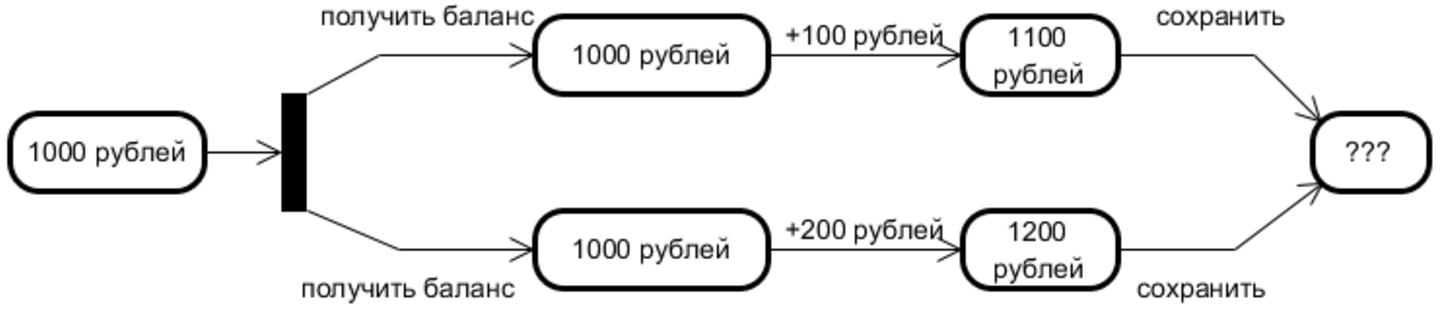
\includegraphics[width=0.9\textwidth]{raceCondition.png}
		\end{center}
	\end{frame}

	\begin{frame}[fragile]
		\frametitle{Маленький пример на race condition}
		\begin{footnotesize}
			\begin{minted}{java}
int[] a = new int[1000];
for (int i = 0; i < a.length; ++i) {
    a[i] = 1;
}

int[] result = new int[1];

for (int i = 0; i < 100; ++i) {
    final int localI = i;
    new Thread(() -> {
        for (int j = localI * 10; j <= (localI + 1) * 10 - 1; ++j) {
            result[0] += a[j];
        }
    }).start();
}

Thread.sleep(100);

System.out.println("Result = " + result[0]);
			\end{minted}
		\end{footnotesize}
	\end{frame}

	\begin{frame}
		\frametitle{Deadlock}
		\begin{center}
			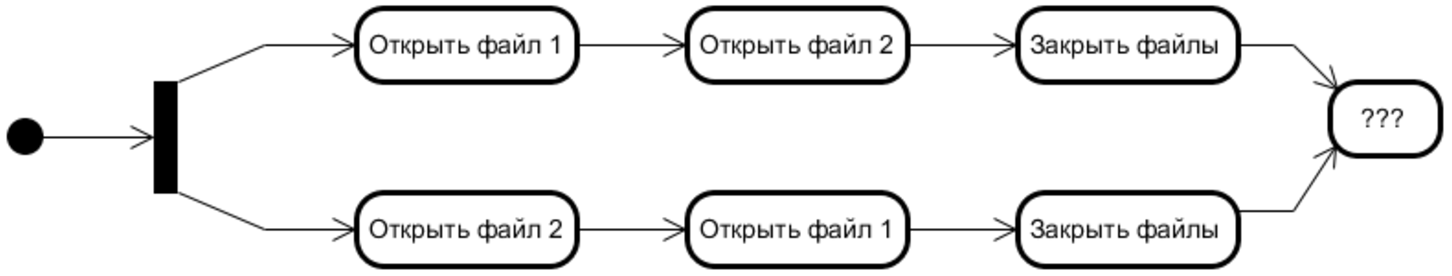
\includegraphics[width=0.9\textwidth]{deadlock.png}
		\end{center}
	\end{frame}

	\begin{frame}[fragile]
		\frametitle{Очень маленький пример на deadlock}
		\begin{footnotesize}
			\begin{minted}{java}
Thread.currentThread().join();
			\end{minted}
		\end{footnotesize}
	\end{frame}

	\begin{frame}
		\frametitle{Пример, потоки в Windows}
		\begin{itemize}
			\item Thread Kernel Object (\textasciitilde1240 байт)
			\item Thread environment block (TEB) (4 Кб)
			\item User-mode stack (1 Мб)
			\item Kernel-mode stack (24 Кб)
		\end{itemize}

		Ещё для каждой dll-ки, загруженной для процесса при старте или остановке потока вызывается DllMain с параметрами DLL\_THREAD\_ATTACH и DLL\_THREAD\_DETACH

		\vspace{3mm}
		Квант времени --- ~20-30 мс, после чего происходит \textit{переключение контекстов}
	\end{frame}

	\begin{frame}
		\frametitle{Как делать не надо}
		\begin{center}
			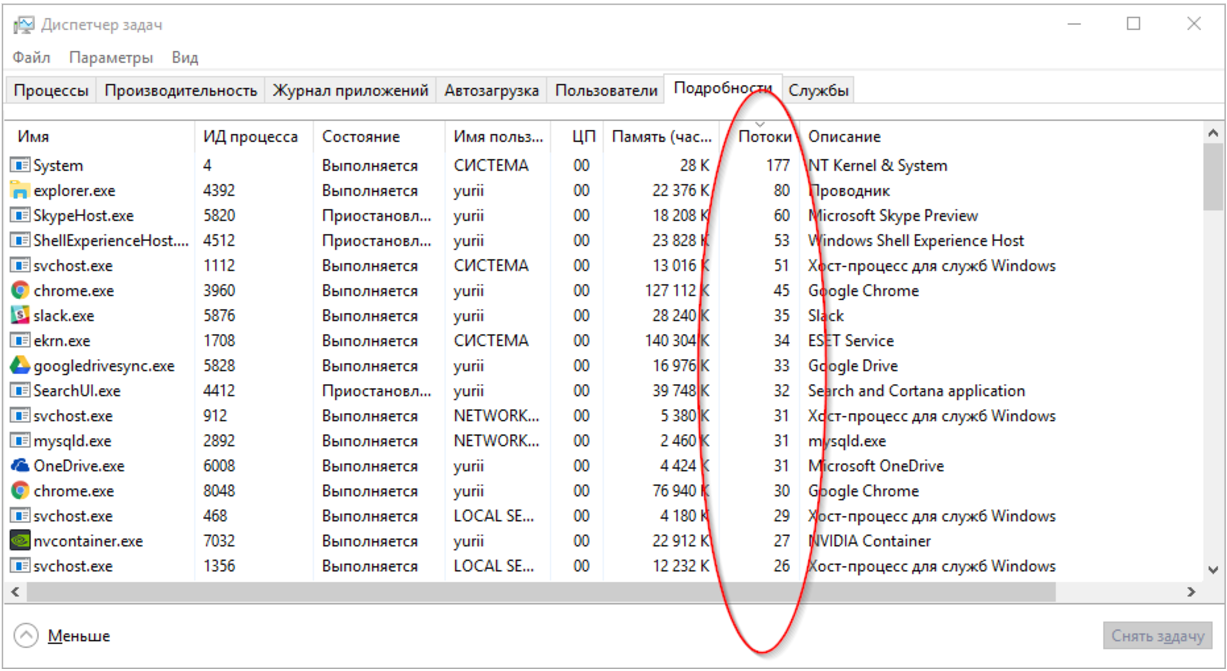
\includegraphics[width=0.9\textwidth]{threadsEverywhere.png}
		\end{center}
	\end{frame}

	\begin{frame}[fragile]
		\frametitle{Задача на пару, многопоточный Lazy}
		Реализовать следующий интерфейс, представляющий ленивое вычисление:
		
		\begin{minted}{java}
public interface Lazy<T> {
    T get();
}
		\end{minted}

		\begin{itemize}
			\item Объект \textit{Lazy} создаётся на основе вычисления (представляемого объектом \textit{Supplier})
			\item Первый вызов \textit{get()} вызывает вычисление и возвращает результат
			\item Повторные вызовы \textit{get()} возвращают \textbf{тот же} объект, что и первый вызов
			\item Вычисление Supplier.get() должно запускаться не более одного раза для однопоточного случая и для ``простого'' многопоточного случая
		\end{itemize}
	\end{frame}

	\begin{frame}
		\frametitle{LazyFactory}
		Создавать объекты надо не вручную, а с помощью класса \textit{LazyFactory}, который должен
		иметь два метода с сигнатурами вида \textit{public static <T> Lazy<T> 
		create...Lazy(Supplier<T>)}, возвращающих три разные реализации \textit{Lazy<T>}:
		\begin{itemize}
			\item Простая версия с гарантией корректной работы в однопоточном режиме (без синхронизации)
			\item Гарантия корректной работы в многопоточном режиме; вычисление не должно производиться более одного раза
			\begin{itemize}
				\item Что-то наподобие многопоточного синглтона
			\end{itemize}
			\item Для многопоточного lock-free режима
			\begin{itemize}
				\item вычисление может производиться > 1 раза, но при этом Lazy.get всегда должен возвращать один и тот же объект (см. AtomicReference/AtomicReferenceFieldUpdater)
			\end{itemize}
		\end{itemize}
	\end{frame}
	
	\begin{frame}
		\frametitle{При этом}
		\begin{itemize}
			\item Ограничение по памяти на каждый \textit{Lazy}-объект: не больше двух полей
			\item \textit{Supplier.get} вправе вернуть \textit{null}
			\item Тесты
			\begin{itemize}
				\item Однопоточные, на разные хорошие и плохие случаи
				\item Многопоточные, на наличие гонок
			\end{itemize}
			\item Делать в командах по два человека
		\end{itemize}
	\end{frame}

	\begin{frame}
		\frametitle{Баллы}
		\begin{itemize}
			\item 1 балл за однопоточную реализацию
			\item 2 балла за многопоточную реализацию с блокировками
			\item 2 балла за многопоточную реализацию с lock-free
			\item 1 балл за многопоточные тесты на гонки (включая требование, что вычисление производится один раз)
			\item -1 балл, если потоки неоправданно мешают друг другу
			\item -1 балл за потенциальные проблемы с порядком операций
		\end{itemize}
	\end{frame}

\end{document}

